\documentclass[aspectratio=169]{beamer}
\usetheme[theme=blue,logo=logowithtextvi]{HUST} 
\DeclareUnicodeCharacter{221E}{\ensuremath{\infty}}

\usepackage[T5]{fontenc}
\usepackage[utf8]{inputenc}
\usepackage{amsmath}
\usepackage{amsfonts}
\usepackage{amssymb}
\usepackage{graphicx}
\usepackage{adjustbox}
\usepackage{xcolor}
\usepackage{tikz}
\usepackage{minted}
\usepackage{tcolorbox}


\usetikzlibrary{positioning,calc,shapes.symbols,matrix,fit,backgrounds,decorations.pathreplacing,arrows.meta}
\definecolor{codeblue}{RGB}{0,90,200}   
\definecolor{codegold}{RGB}{210,160,0}
\definecolor{HUSTBlue}{RGB}{0,51,102}

\setminted{
	breaklines=false,
	autogobble=false,
	obeytabs=true,
	tabsize=2,
	linenos=true,
	showspaces=false,
	space=~,
	baselinestretch=1,
	fontsize=\normalsize,
	rulecolor=\color{black}
}

\newcommand{\placecontent}[4]{%
	\tikz[remember picture,overlay]
	\node[anchor=north west]
	at ([xshift=#1,yshift=-#2]current page.north west)
	{\parbox{#3}{#4}};
}

\graphicspath{{./week 14 resources/}}

\title{\huge CẤU TRÚC DỮ LIỆU VÀ GIẢI THUẬT}
\author{SoICT - HUST}
\date{}

\begin{document}
	
	% 2 slides đầu tiên:
	\HUSTInsertBrandSlide
	\HUSTInsertThemeSlide
	
	% Slide tiêu đề
	{\HUSTUseBackground{onelove.pdf}
		\begin{frame}
			\ifdefstring{\insertaspectratio}{169}{
				\HUSTCornerImage[0.14]{assets/logo/soict_vi_h.pdf}
				\placecontent{0.5cm}{0.33\paperheight}{0.85\paperwidth}{
					\color{\HUSTFrameTitleTextColor}\bfseries\fontsize{22pt}{30pt}\selectfont
					\inserttitle
				}
				\placecontent{0.5cm}{0.50\paperheight}{0.8\paperwidth}{
					\color{\HUSTFrameTitleTextColor}\fontsize{14pt}{14pt}\selectfont
					%Bài học
					\textbf{\large TUẦN 14: ĐỒ THỊ(PHẦN 1)}\\
				}
			}{}
		\end{frame}
	}
	
	% Outline
	\AtBeginSection[]
	{
		\begin{frame}<beamer>
			\frametitle{NỘI DUNG}
			\tableofcontents[currentsection]
		\end{frame}
	}
	
	%Nội dung chính trong slides
	\section{Nhắc lại khái niệm cơ bản về đồ thị}
	\begin{frame}[t]{NHẮC LẠI KHÁI NIỆM CƠ BẢN VỀ ĐỒ THỊ}
		\small
		\setlength{\leftmargini}{-1.2em}
		
		\begin{itemize}
			\item \textbf{Đồ thị} là cấu trúc bao gồm các thực thể (còn gọi là \textit{đỉnh})
			và liên kết giữa các thực thể (còn gọi là \textit{cạnh} hoặc \textit{cung}).
			\item Ký hiệu đồ thị: $G=(V,E)$, trong đó $V$ là tập đỉnh và $E$ là tập cạnh (cung).
			\item Với $(u,v)\in E$: ta nói $u$ và $v$ là hai đỉnh kề nhau.
		\end{itemize}
		
		
\begingroup
\colorlet{GraphBorder}{HUSTBlue!55}
\colorlet{GraphNode}{HUSTBlue!45}
\setlength{\fboxsep}{2pt} % (3pt -> 2pt) giảm padding => cạnh dưới lên

\centering
\fcolorbox{GraphBorder}{white}{%
	\begin{minipage}{0.90\textwidth}
		\begin{columns}[T,onlytextwidth]
			
			%================ LEFT: UNDIRECTED =================
			\column{0.48\textwidth}
			\centering
			
			\begin{tikzpicture}[scale=0.85] % GIỮ NGUYÊN
				\tikzset{
					v/.style={circle, draw=GraphNode, fill=GraphNode,
						minimum size=8mm, inner sep=0pt, text=white, font=\bfseries}, % GIỮ NGUYÊN
					e/.style={draw=GraphBorder, line width=0.9pt}
				}
				
				\node[v] (n5) at (0,1.2) {5};
				\node[v] (n2) at (1.6,1.2) {2};
				\node[v] (n4) at (1.6,0) {4};
				\node[v] (n3) at (0,0) {3};
				\node[v] (n1) at (-1.3,0.6) {1};
				
				\draw[e] (n5)--(n2);
				\draw[e] (n2)--(n4);
				\draw[e] (n4)--(n3);
				\draw[e] (n3)--(n5);
				\draw[e] (n1)--(n5);
				\draw[e] (n1)--(n3);
			\end{tikzpicture}
			
			\vspace{-0.10cm} % siết khoảng cách hình -> chữ
			
			\begin{minipage}[t]{\linewidth}
				\raggedright
				\textbf{Đồ thị vô hướng}\vspace{-0.15cm}
				
				{\setlength{\leftmargini}{1.2em}
					\setlength{\topsep}{0.1em}
					\setlength{\itemsep}{0.15em}
					\setlength{\parsep}{0pt}
					\setlength{\partopsep}{0pt}
					\begin{itemize}
						\item $V=\{1,2,3,4,5\}$
						\item {\scriptsize$
							\begin{aligned}[t]
								E=\{&(1,3),(1,5),(2,4),(2,5),\\
								&(3,4),(3,5)\}
							\end{aligned}
							$}
				\end{itemize}}
			\end{minipage}
			
			%================ MID DIVIDER =================
			\column{0.04\textwidth}
			\centering
			\textcolor{GraphBorder}{\rule{0.6pt}{4.20cm}} % (4.8cm -> 4.2cm) cái này kéo cạnh dưới lên mạnh nhất
			
			%================ RIGHT: DIRECTED =================
			\column{0.48\textwidth}
			\centering
			
			\begin{tikzpicture}[scale=0.85] % GIỮ NGUYÊN
				\tikzset{
					v/.style={circle, draw=GraphNode, fill=GraphNode,
						minimum size=8mm, inner sep=0pt, text=white, font=\bfseries}, % GIỮ NGUYÊN
					a/.style={->, draw=GraphBorder, line width=0.9pt}
				}
				
				\node[v] (n1) at (-1.6,0.6) {1};
				\node[v] (n6) at (0,1.25) {6};
				\node[v] (n3) at (0,0) {3};
				\node[v] (n2) at (1.6,1.25) {2};
				\node[v] (n4) at (1.6,0) {4};
				\node[v] (n5) at (3.0,0.6) {5};
				
				\draw[a] (n1) -> (n6);
				\draw[a] (n1) -> (n3);
				\draw[a] (n6) -> (n2);
				\draw[a] (n6) -> (n3);
				\draw[a] (n3) -> (n4);
				\draw[a] (n2) -> (n4);
				\draw[a] (n2) -> (n5);
				\draw[a] (n4) -> (n5);
			\end{tikzpicture}
			
			\vspace{-0.10cm} % siết khoảng cách hình -> chữ
			
			\begin{minipage}[t]{\linewidth}
				\raggedright
				\textbf{Đồ thị có hướng}\vspace{-0.15cm}
				
				{\setlength{\leftmargini}{1.2em}
					\setlength{\topsep}{0.1em}
					\setlength{\itemsep}{0.15em}
					\setlength{\parsep}{0pt}
					\setlength{\partopsep}{0pt}
					\begin{itemize}
						\item $V=\{1,2,3,4,5,6\}$
						\item {\scriptsize$
							\begin{aligned}[t]
								E=\{&(1,3),(1,6),(6,2),(6,3),\\
								&(2,4),(2,5),(3,4),(4,5)\}
							\end{aligned}
							$}
				\end{itemize}}
			\end{minipage}
			
		\end{columns}
	\end{minipage}%
}
\endgroup

	\end{frame}
	
	\begin{frame}[t]{NHẮC LẠI KHÁI NIỆM CƠ BẢN VỀ ĐỒ THỊ}
		\small

		\setlength{\leftmargini}{-1.2em}
		
		\begin{itemize}
			\item Cho $G=(V,E)$ là một đồ thị.
			\begin{itemize}
				\item \textbf{Đường đi} từ đỉnh $s$ đến đỉnh $t$ trên đồ thị là dãy các đỉnh
				$v_1, v_2, \ldots, v_k$ trong đó
				\begin{itemize}
					\item $s=v_1,\; t=v_k$.
					\item $(v_i, v_{i+1}) \in E$ \quad $(i=1,\ldots,k-1)$.
				\end{itemize}
				
				\item \textbf{Chu trình} là đường đi trong đó đỉnh đầu và cuối trùng nhau.
			\end{itemize}
			
			\item \textbf{Đồ thị vô hướng} $G$ được gọi là \textbf{liên thông} nếu giữa $2$ đỉnh bất kỳ của $G$
			luôn có đường đi giữa chúng.
		\end{itemize}
	\end{frame}
	
	
\section{Cấu trúc dữ liệu biểu diễn đồ thị}

	\begin{frame}[t]{CẤU TRÚC DỮ LIỆU BIỂU DIỄN ĐỒ THỊ}
		\small
		\setlength{\leftmargini}{-1.2em}
		
		\begin{itemize}
			\item Ma trận kề, ma trận trọng số
			\item Danh sách kề
			\item Danh sách cạnh
		\end{itemize}
	\end{frame}
	
	\begin{frame}[t]{CẤU TRÚC DỮ LIỆU BIỂU DIỄN ĐỒ THỊ}
		\small
		\setlength{\leftmargini}{-1.2em}
		
		\begin{itemize}
			\item \textbf{Ma trận kề, ma trận trọng số}
		\end{itemize}
		
		\centering
		
		\begingroup
		\colorlet{GraphLine}{HUSTBlue!70}
		\colorlet{ArrowBlue}{HUSTBlue!75}
		
		\begin{tikzpicture}[font=\small, ampersand replacement=\&]
			%==================== styles ====================
			\tikzset{
				v/.style={circle, draw=GraphLine, line width=1pt,
					minimum size=7mm, inner sep=0pt, font=\bfseries},
				e/.style={draw=GraphLine, line width=1pt},
				warrow/.style={-{Stealth[length=5mm,width=5mm]}, draw=ArrowBlue, line width=3pt},
				mcell/.style={draw=black, minimum size=6.0mm, inner sep=0pt},
				mlabel/.style={font=\bfseries}
			}
			
			%========================================================
			%  CỤM 2 ĐỒ THỊ + 2 MŨI TÊN (dịch đồng thời)
			%========================================================
			\begin{scope}[xshift=-0.9cm, yshift=-0.25cm] % <-- chỉnh nếu muốn
				
				%---------------- TOP GRAPH ----------------
				\begin{scope}[shift={(0,0)}]
					\node[v] (a1) at (0,1.4) {1};
					\node[v] (a2) at (2.2,1.4) {2};
					\node[v] (a3) at (0,0) {3};
					\node[v] (a4) at (2.2,0) {4};
					
					\draw[e] (a1)--(a2);
					\draw[e] (a1)--(a3);
					\draw[e] (a3)--(a4);
					\draw[e] (a2)--(a4);
					\draw[e] (a1)--(a4);
				\end{scope}
				
				\draw[warrow] (3.1,0.7) -- (4.3,0.7);
				
				%---------------- BOTTOM GRAPH ----------------
				\begin{scope}[shift={(0,-3.0)}]
					\node[v] (b1) at (0,1.4) {1};
					\node[v] (b2) at (2.2,1.4) {2};
					\node[v] (b3) at (0,0) {3};
					\node[v] (b4) at (2.2,0) {4};
					
					\draw[e] (b1)-- node[above, font=\bfseries] {5} (b2);
					\draw[e] (b1)-- node[left,  font=\bfseries] {2} (b3);
					\draw[e] (b3)-- node[below, font=\bfseries] {6} (b4);
					\draw[e] (b2)-- node[right, font=\bfseries] {4} (b4);
					\draw[e] (b1)-- node[above right, font=\bfseries] {1} (b4);
				\end{scope}
				
				\draw[warrow] (3.1,-2.3) -- (4.3,-2.3);
				
			\end{scope}
			
			%========================================================
			%  2 MA TRẬN (thu nhỏ bằng scale)
			%========================================================
			\begin{scope}[shift={(5.2,0.15)}, scale=0.85, transform shape]
				\scriptsize
				\matrix (M1) [matrix of nodes,
				nodes={mcell},
				column sep=-\pgflinewidth,
				row sep=-\pgflinewidth] {
					0 \& 1 \& 1 \& 1 \\
					1 \& 0 \& 0 \& 1 \\
					1 \& 0 \& 0 \& 1 \\
					1 \& 1 \& 1 \& 0 \\
				};
				
				\node[mlabel, above=1mm of M1-1-1] {1};
				\node[mlabel, above=1mm of M1-1-2] {2};
				\node[mlabel, above=1mm of M1-1-3] {3};
				\node[mlabel, above=1mm of M1-1-4] {4};
				
				\node[mlabel, left=1mm of M1-1-1] {1};
				\node[mlabel, left=1mm of M1-2-1] {2};
				\node[mlabel, left=1mm of M1-3-1] {3};
				\node[mlabel, left=1mm of M1-4-1] {4};
			\end{scope}
			
			\begin{scope}[shift={(5.2,-2.85)}, scale=0.85, transform shape]
				\scriptsize
				\matrix (M2) [matrix of nodes,
				nodes={mcell},
				column sep=-\pgflinewidth,
				row sep=-\pgflinewidth] {
					0 \& 5 \& 2 \& 1 \\
					5 \& 0 \& 0 \& 4 \\
					2 \& 0 \& 0 \& 6 \\
					1 \& 4 \& 6 \& 0 \\
				};
				
				\node[mlabel, above=1mm of M2-1-1] {1};
				\node[mlabel, above=1mm of M2-1-2] {2};
				\node[mlabel, above=1mm of M2-1-3] {3};
				\node[mlabel, above=1mm of M2-1-4] {4};
				
				\node[mlabel, left=1mm of M2-1-1] {1};
				\node[mlabel, left=1mm of M2-2-1] {2};
				\node[mlabel, left=1mm of M2-3-1] {3};
				\node[mlabel, left=1mm of M2-4-1] {4};
			\end{scope}
			
		\end{tikzpicture}
		\endgroup
	\end{frame}
	
	\begin{frame}[t]{CẤU TRÚC DỮ LIỆU BIỂU DIỄN ĐỒ THỊ}
		\small
		\setlength{\leftmargini}{-1.2em}
		
		\begin{itemize}
			\item \textbf{Danh sách kề}
			\begin{itemize}
				\item \textbf{A[v]}: danh sách các đỉnh (hoặc cạnh/cung đối với đồ thị trọng số) kề với đỉnh $v$
			\end{itemize}
		\end{itemize}
		
		\centering
		
		\begingroup
		\colorlet{GraphLine}{HUSTBlue!70}
		\colorlet{ArrowBlue}{HUSTBlue!75}
		
		% width cố định cho 2 khung (bằng nhau) nhưng không quá thừa
		
		\begin{tikzpicture}[font=\small]
			\tikzset{
				v/.style={circle, draw=GraphLine, line width=1.0pt, fill=white,
					minimum size=7mm, inner sep=0pt, font=\bfseries},
				e/.style={draw=GraphLine, line width=1.0pt},
				warrow/.style={-{Stealth[length=4.2mm,width=4.2mm]}, draw=ArrowBlue, line width=2.6pt},
				abox/.style={draw=GraphLine, line width=0.9pt, fill=white,
					inner xsep=4pt, inner ysep=1.2pt, align=left, text width=5.3cm}
			}
			\def\bl{\textcolor{HUSTBlue}{\scriptsize$\bullet$}\,}
			
			%==================== TOP ROW ====================
			\begin{scope}[xshift=-0.55cm, yshift=0.05cm]
				\node[v] (a1) at (0,1.35) {1};
				\node[v] (a2) at (2.2,1.35) {2};
				\node[v] (a3) at (0,0) {3};
				\node[v] (a4) at (2.2,0) {4};
				
				\draw[e] (a1)--(a2);
				\draw[e] (a1)--(a3);
				\draw[e] (a3)--(a4);
				\draw[e] (a2)--(a4);
				\draw[e] (a1)--(a4);
				
				\draw[warrow] (3.15,0.675) -- (4.25,0.675);
				
				\node[abox, anchor=west] at (4.55,0.675) {%
					\scriptsize
					\setlength{\tabcolsep}{0pt}
					\renewcommand{\arraystretch}{1.25}
					\begin{tabular}{@{}l@{}}
						\bl $\mathrm{A}[1]=[2,3,4]$\\
						\bl $\mathrm{A}[2]=[1,4]$\\
						\bl $\mathrm{A}[3]=[1,4]$\\
						\bl $\mathrm{A}[4]=[1,2,3]$\\
					\end{tabular}
				};
			\end{scope}
			
			%==================== BOTTOM ROW ====================
			\begin{scope}[xshift=-0.55cm, yshift=-3.05cm]
				\node[v] (b1) at (0,1.35) {1};
				\node[v] (b2) at (2.2,1.35) {2};
				\node[v] (b3) at (0,0) {3};
				\node[v] (b4) at (2.2,0) {4};
				
				\draw[e] (b1)-- node[above, font=\bfseries\scriptsize] {5} (b2);
				\draw[e] (b1)-- node[left,  font=\bfseries\scriptsize] {2} (b3);
				\draw[e] (b3)-- node[below, font=\bfseries\scriptsize] {6} (b4);
				\draw[e] (b2)-- node[right, font=\bfseries\scriptsize] {4} (b4);
				\draw[e] (b1)-- node[pos=0.55, above right, font=\bfseries\scriptsize] {1} (b4);
				
				\draw[warrow] (3.15,0.675) -- (4.25,0.675);
				
				\node[abox, anchor=west] at (4.55,0.675) {%
					\scriptsize
					\setlength{\tabcolsep}{0pt}
					\renewcommand{\arraystretch}{1.25}
					\begin{tabular}{@{}l@{}}
						\bl $\mathrm{A}[1]=[(1,2,5),(1,3,2),(1,4,1)]$\\
						\bl $\mathrm{A}[2]=[(1,2,5),(2,4,4)]$\\
						\bl $\mathrm{A}[3]=[(1,3,2),(3,4,6)]$\\
						\bl $\mathrm{A}[4]=[(1,4,1),(2,4,4),(3,4,6)]$\\
					\end{tabular}
				};
			\end{scope}
			
		\end{tikzpicture}
		\endgroup
		
	\end{frame}
	
	\begin{frame}[t]{CẤU TRÚC DỮ LIỆU BIỂU DIỄN ĐỒ THỊ}
		\small
		\setlength{\leftmargini}{-1.2em}
		
		\begin{itemize}
			\item \textbf{Danh sách cạnh}
			\begin{itemize}
				\item \textbf{E}: danh sách các cạnh/cung của đồ thị
			\end{itemize}
		\end{itemize}
		
		\centering
		
		\begingroup
		\colorlet{GraphLine}{HUSTBlue!70}
		\colorlet{ArrowBlue}{HUSTBlue!75}
		
		\begin{tikzpicture}[font=\small]
			\tikzset{
				v/.style={circle, draw=GraphLine, line width=1.0pt, fill=white,
					minimum size=7mm, inner sep=0pt, font=\bfseries},
				e/.style={draw=GraphLine, line width=1.0pt},
				warrow/.style={-{Stealth[length=4.2mm,width=4.2mm]}, draw=ArrowBlue, line width=2.6pt},
				ebox/.style={draw=GraphLine, line width=0.9pt, fill=white,
					inner xsep=6pt, inner ysep=3pt, align=left, text width=7.2cm}
			}
			
			%==================== TOP ROW (unweighted) ====================
			\begin{scope}[xshift=-0.55cm, yshift=0.05cm]
				% graph
				\node[v] (a1) at (0,1.35) {1};
				\node[v] (a2) at (2.2,1.35) {2};
				\node[v] (a3) at (0,0) {3};
				\node[v] (a4) at (2.2,0) {4};
				
				\draw[e] (a1)--(a2);
				\draw[e] (a1)--(a3);
				\draw[e] (a3)--(a4);
				\draw[e] (a2)--(a4);
				\draw[e] (a1)--(a4);
				
				% arrow
				\draw[warrow] (3.15,0.675) -- (4.25,0.675);
				
				% box
				\node[ebox, anchor=west] at (4.55,0.675) {%
					\scriptsize
					\setlength{\tabcolsep}{0pt}
					\renewcommand{\arraystretch}{1.15}
					\begin{tabular}{@{}l@{}}
						Danh sách cạnh: $E=[(1,2),(1,3),(1,4),(2,4),$\\
						\hspace*{2.35cm}$(3,4)]$
					\end{tabular}
				};
			\end{scope}
			
			%==================== BOTTOM ROW (weighted) ====================
			\begin{scope}[xshift=-0.55cm, yshift=-3.05cm]
				% graph
				\node[v] (b1) at (0,1.35) {1};
				\node[v] (b2) at (2.2,1.35) {2};
				\node[v] (b3) at (0,0) {3};
				\node[v] (b4) at (2.2,0) {4};
				
				\draw[e] (b1)-- node[above, font=\bfseries\scriptsize] {5} (b2);
				\draw[e] (b1)-- node[left,  font=\bfseries\scriptsize] {2} (b3);
				\draw[e] (b3)-- node[below, font=\bfseries\scriptsize] {6} (b4);
				\draw[e] (b2)-- node[right, font=\bfseries\scriptsize] {4} (b4);
				\draw[e] (b1)-- node[pos=0.55, above right, font=\bfseries\scriptsize] {1} (b4);
				
				% arrow
				\draw[warrow] (3.15,0.675) -- (4.25,0.675);
				
				% box
				\node[ebox, anchor=west] at (4.55,0.675) {%
					\scriptsize
					\setlength{\tabcolsep}{0pt}
					\renewcommand{\arraystretch}{1.15}
					\begin{tabular}{@{}l@{}}
						Danh sách cạnh kèm trọng số trên cạnh\\
						$E=[(1,2,5),(1,3,2),(1,4,1),(2,4,4),(3,4,6)]$
					\end{tabular}
				};
			\end{scope}
			
		\end{tikzpicture}
		\endgroup
	\end{frame}
	
\section{Duyệt đồ thị}
	% ====== SLIDE: DUYỆT ĐỒ THỊ (DFS) - TRÁI SÁT TRÁI, PHẢI SÁT PHẢI ======
	\begin{frame}[t]{DUYỆT ĐỒ THỊ}
		\small
		\setlength{\leftmargini}{-1.2em}
		
		\begin{itemize}
			\item Duyệt đồ thị theo chiều sâu: thăm các đỉnh của đồ thị, mỗi đỉnh đúng 1 lần
			\item $A[v]$: danh sách các đỉnh kề với $v$
		\end{itemize}
		
		\vspace{0.25cm}
		
		% --- kéo điểm bắt đầu từ "lề text" ra đúng mép trái trang
		\noindent\hspace*{-\dimexpr(\paperwidth-\textwidth)/2\relax}%
		\begin{minipage}[t]{\paperwidth}
			
			% ===== chỉnh 2 giá trị này để "kéo vào trong" & "giảm gap giữa 2 khung" =====
			\def\outerinset{3mm} % lề trong 2 bên (tăng lên nếu còn tràn)
			\def\midgap{2mm}     % khoảng cách giữa 2 khung (giảm xuống nếu muốn sát hơn)
			
			\hspace*{\outerinset}%
			% ===== LEFT =====
			\begin{minipage}[t]{0.45\paperwidth}
				\begin{tcolorbox}[
					colback=white,
					colframe=blue!60,
					boxrule=0.6pt,
					arc=0pt,
					left=-1pt,right=2pt,top=-1pt,bottom=-1pt,
					height=0.48\textheight,
					valign=top,
					fontupper=\ttfamily\scriptsize
					]
					\begin{tabbing}
						\hspace{1em}\=\hspace{1em}\=\hspace{1em}\=\kill
						\textbf{DFS}(u, A)\{// duyệt theo chiều sâu từ đỉnh u\\[2pt]
						\> visited[u] = true; \ \ \ // Thăm đỉnh u;\\[2pt]
						\> for v in A[u] do \{\\[2pt]
						\>\> if visited[v] = false then \{\\[2pt]
						\>\>\> DFS(v, A);\\[2pt]
						\>\> \}\\[2pt]
						\> \}\\[2pt]
						\}\\
					\end{tabbing}
				\end{tcolorbox}
			\end{minipage}%
			\hspace*{\midgap}%
			% ===== RIGHT =====
			\begin{minipage}[t]{0.45\paperwidth}
				\begin{tcolorbox}[
					colback=white,
					colframe=blue!60,
					boxrule=0.6pt,
					arc=0pt,
					left=-1pt,right=-1pt,top=-1pt,bottom=-1pt,
					height=0.48\textheight,
					valign=top,
					fontupper=\ttfamily\scriptsize
					]
					\begin{tabbing}
						\hspace{1em}\=\hspace{1em}\=\hspace{1em}\=\kill
						\textbf{DFS}(G = (V, A))\{// duyệt theo chiều sâu trên G\\[1pt]
						\> for v in V do visited[v] = false;\\[1pt]
						\> for v in V do \{\\[2pt]
						\>\> if visited[v] = false then \{\\[1pt]
						\>\>\> DFS(v, A);\\[1pt]
						\>\> \}\\[1pt]
						\> \}\\[1pt]
						\}\\
					\end{tabbing}
				\end{tcolorbox}
			\end{minipage}%
			\hspace*{\outerinset}
			
		\end{minipage}
	\end{frame}
	
\begin{frame}[t]{DUYỆT ĐỒ THỊ}
	\small
	\setlength{\leftmargini}{-1.2em}
	\newlength{\LBoxShift}
	\setlength{\LBoxShift}{6mm} % tăng lên => khung trái dịch trái nhiều hơn
	
	\begin{columns}[T,onlytextwidth]
		
		% ===================== LEFT COLUMN =====================
		\begin{column}{0.46\textwidth}
			\begin{itemize}
				\item Duyệt đồ thị theo chiều rộng: thăm các đỉnh của đồ thị, mỗi đỉnh đúng 1 lần
				\item $A[v]$: danh sách các đỉnh kề với $v$
			\end{itemize}
					
			% --- CHỈ DỊCH KHUNG, KHÔNG DỊCH BULLET ---
			\noindent\hspace*{-\LBoxShift}%
			\begin{minipage}[t]{\dimexpr\linewidth+\LBoxShift\relax}
				\begin{tcolorbox}[
					colback=white,
					colframe=blue!60,
					boxrule=0.6pt,
					arc=0pt,
					boxsep=0pt,
					left=3pt,right=3pt,top=3pt,bottom=3pt,
					height=0.46\textheight,
					valign=top,
					fontupper=\ttfamily\scriptsize
					]
					\begin{tabbing}
						\hspace{1em}\=\hspace{1em}\=\hspace{1em}\=\hspace{1em}\=\hspace{1.2em}\=\kill
						\textbf{BFS}(G = (V, A))\{//duyệt theo chiều rộng trên G\\[4pt]
						\> for v in V do visited[v] = false;\\[8pt]
						\> for v in V do \{\\[4pt]
						\>\> if visited[v] = false then \{\\[4pt]
						\>\>\> BFS(v, A);\\[4pt]
						\>\> \}\\[4pt]
						\> \}\\[2pt]
						\}\\
					\end{tabbing}
				\end{tcolorbox}
			\end{minipage}
		\end{column}
		
		% ===================== RIGHT COLUMN =====================
		\begin{column}{0.52\textwidth}
			\begin{tcolorbox}[
				colback=white,
				colframe=blue!60,
				boxrule=0.6pt,
				arc=0pt,
				boxsep=0pt,
				left=3pt,right=3pt,top=3pt,bottom=3pt,
				height=0.635\textheight,
				valign=top,
				fontupper=\ttfamily\scriptsize
				]
				\begin{tabbing}
					\hspace{1em}\=\hspace{1em}\=\hspace{1em}\=\hspace{1em}\=\hspace{1em}\=\kill
					\textbf{BFS}(u, A) \{// duyệt theo chiều rộng từ đỉnh u\\[8pt]
					\> Q = hàng đợi rỗng;\\[10pt]
					\> Q.push(u);\ \ visited[u] = true; //thăm đỉnh u\\[3pt]
					\> while Q not empty do \{\\[3pt]
					\>\> v = Q.pop();\\[3pt]
					\>\> for x in A[v] do\\[3pt]
					\>\>\> if visited[x] = false then \{\\[3pt]
					\>\>\>\> Q.push(x);\ visited[x] = true; //thăm x\\[3pt]
					\>\>\> \}\\[3pt]
					\> \}\\[3pt]
					\}\\
				\end{tabbing}
			\end{tcolorbox}
		\end{column}
		
	\end{columns}
\end{frame}

\section{Tìm thành phần liên thông đồ thị}

\begin{frame}[t]{TÌM THÀNH PHẦN LIÊN THÔNG CỦA ĐỒ THỊ}
	\small
	\setlength{\leftmargini}{-1.2em}
	
	\begin{columns}[T,onlytextwidth]
		% ================= LEFT =================
		\begin{column}{0.68\textwidth}
			\begin{itemize}
				\item Mô tả bài toán
				\begin{itemize}
					\item Cho đồ thị vô hướng $G = (V, A)$ trong đó
					\begin{itemize}
						\item $V$ là tập đỉnh
						\item $A$ là cấu trúc danh sách kề: $A[v]$ là danh sách các đỉnh kề với $v$
					\end{itemize}
					\item Cần tìm các thành phần liên thông của $G$
				\end{itemize}
				
				
				\item Thuật toán:
				\begin{itemize}
					\item Áp dụng duyệt theo chiều sâu (hoặc duyệt theo chiều rộng) trên $G$
					\item DFS$(u)$ cho phép thăm tất cả các đỉnh thuộc cùng thành phần liên thông với $u$
				\end{itemize}
			\end{itemize}
		\end{column}
		
		% ================= RIGHT =================
		\begin{column}{0.32\textwidth}
			\centering
			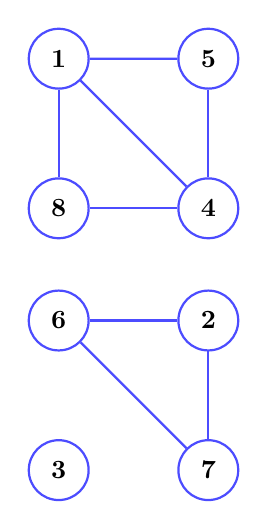
\begin{tikzpicture}[scale=0.95, every node/.style={transform shape}]
				\tikzset{
					vertex/.style={circle, draw=blue!70, thick, minimum size=8mm, inner sep=0pt, font=\bfseries},
					edge/.style={draw=blue!70, thick}
				}
				
				% ---- Component 1 (1,5,8,4) ----
				\node[vertex] (n1) at (0,3) {1};
				\node[vertex] (n5) at (2,3) {5};
				\node[vertex] (n8) at (0,1) {8};
				\node[vertex] (n4) at (2,1) {4};
				
				\draw[edge] (n1) -- (n5);
				\draw[edge] (n1) -- (n8);
				\draw[edge] (n8) -- (n4);
				\draw[edge] (n5) -- (n4);
				\draw[edge] (n1) -- (n4);
				
				% ---- Component 2 (6,2,7) ----
				\node[vertex] (n6) at (0,-0.5) {6};
				\node[vertex] (n2) at (2,-0.5) {2};
				\node[vertex] (n7) at (2,-2.5) {7};
				
				\draw[edge] (n6) -- (n2);
				\draw[edge] (n2) -- (n7);
				\draw[edge] (n6) -- (n7);
				
				% ---- Isolated vertex 3 ----
				\node[vertex] (n3) at (0,-2.5) {3};
			\end{tikzpicture}
		\end{column}
	\end{columns}
\end{frame}

\begin{frame}[t]{TÌM THÀNH PHẦN LIÊN THÔNG CỦA ĐỒ THỊ}
	\small
	\setlength{\leftmargini}{-1.2em}
	
	\begin{itemize}
		\item nbCC: số thành phần liên thông của $G$
		\item $C[v]$: chỉ số (chạy từ $1$ đến nbCC) của thành phần liên thông chứa đỉnh $v$
	\end{itemize}

	
	% --- kéo điểm bắt đầu từ "lề text" ra đúng mép trái trang
	\noindent\hspace*{-\dimexpr(\paperwidth-\textwidth)/2\relax}%
	\begin{minipage}[t]{\paperwidth}
		
		% ===== chỉnh 2 giá trị này để kéo vào trong & giảm gap =====
		\def\outerinset{3mm}
		\def\midgap{2mm}
		
		\hspace*{\outerinset}%
		% ================= LEFT =================
		\begin{minipage}[t]{0.45\paperwidth}
			\begin{tcolorbox}[
				colback=white,
				colframe=blue!60,
				boxrule=0.6pt,
				arc=0pt,
				boxsep=0pt,
				left=3pt,right=3pt,top=3pt,bottom=3pt,
				height=0.52\textheight,
				valign=top,
				fontupper=\ttfamily\scriptsize
				]
				\begin{tabbing}
					\hspace{1em}\=\hspace{1em}\=\hspace{1em}\=\hspace{1em}\=\kill
					\textbf{DFS}(u, A) \{// duyệt theo chiều sâu từ đỉnh u\\[4pt]
					
					\> visited[u] = true; \ \ // Thăm đỉnh u;\\[2pt]
					\> C[u] = nbCC;\\[2pt]
					
					\> for v in A[u] do \{\\[2pt]
					\>\> if visited[v] = false then \{\\[2pt]
					\>\>\> DFS(v, A);\\[2pt]
					\>\> \}\\[2pt]
					\> \}\\[2pt]
					\}\\
				\end{tabbing}
			\end{tcolorbox}
		\end{minipage}%
		\hspace*{\midgap}%
		% ================= RIGHT =================
		\begin{minipage}[t]{0.45\paperwidth}
			\begin{tcolorbox}[
				colback=white,
				colframe=blue!60,
				boxrule=0.6pt,
				arc=0pt,
				boxsep=0pt,
				left=3pt,right=3pt,top=3pt,bottom=3pt,
				height=0.52\textheight,
				valign=top,
				fontupper=\ttfamily\scriptsize
				]
				\begin{tabbing}
					\hspace{1em}\=\hspace{1em}\=\hspace{1em}\=\hspace{1em}\=\kill
					\textbf{DFS}(G = (V, A)) \{// duyệt theo chiều sâu trên G\\[4pt]
					
					\> for v in V do visited[v] = false;\\[2pt]
					\> nbCC = 0;\\[2pt]
					
					\> for v in V do \{\\[4pt]
					\>\> if visited[v] = false then \{\\[2pt]
					\>\>\> nbCC = nbCC + 1;\\[2pt]
					\>\>\> DFS(v, A);\\[2pt]
					\>\> \}\\[2pt]
					\> \}\\[2pt]
					\}\\
				\end{tabbing}
			\end{tcolorbox}
		\end{minipage}%
		\hspace*{\outerinset}
		
	\end{minipage}
\end{frame}

\begin{frame}[t]{TÌM THÀNH PHẦN LIÊN THÔNG CỦA ĐỒ THỊ}
	\small
	\setlength{\leftmargini}{-1.2em}
	
	\begin{columns}[T,onlytextwidth]
		
		% ===================== COL 1: TEXT =====================
		\begin{column}{0.39\textwidth}
			\begin{itemize}
				\item Minh họa với ngôn ngữ C
				
				\item Dữ liệu
				\begin{itemize}
					\item Dòng 1: chứa 2 số nguyên dương $n$ và $m$ tương ứng là số đỉnh và số cạnh
					\item Dòng $i + 1$ $(i=1,2,\ldots,m)$: chứa 2 số nguyên dương $u$ và $v$ là 2 đầu mút của cạnh thứ $i$
				\end{itemize}
				
				\item Kết quả
				\begin{itemize}
					\item Hiển thị danh sách các đỉnh của mỗi thành	phần liên thông tìm được trên 1 dòng
				\end{itemize}
			\end{itemize}
		\end{column}
		
		% ===================== COL 2: GRAPH =====================
		\begin{column}{0.23\textwidth}
			\centering
			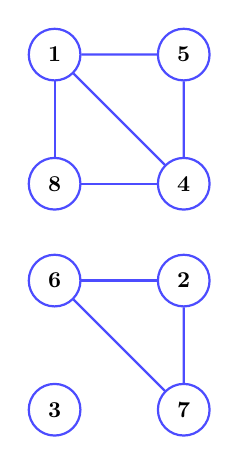
\begin{tikzpicture}[scale=0.82, every node/.style={transform shape}]
				\tikzset{
					vertex/.style={circle, draw=blue!70, thick, minimum size=8mm, inner sep=0pt, font=\bfseries},
					edge/.style={draw=blue!70, thick}
				}
				
				% Component 1
				\node[vertex] (n1) at (0,3) {1};
				\node[vertex] (n5) at (2,3) {5};
				\node[vertex] (n8) at (0,1) {8};
				\node[vertex] (n4) at (2,1) {4};
				
				\draw[edge] (n1)--(n5);
				\draw[edge] (n1)--(n8);
				\draw[edge] (n8)--(n4);
				\draw[edge] (n5)--(n4);
				\draw[edge] (n1)--(n4);
				
				% Component 2
				\node[vertex] (n6) at (0,-0.5) {6};
				\node[vertex] (n2) at (2,-0.5) {2};
				\node[vertex] (n7) at (2,-2.5) {7};
				
				\draw[edge] (n6)--(n2);
				\draw[edge] (n2)--(n7);
				\draw[edge] (n6)--(n7);
				
				% Isolated
				\node[vertex] (n3) at (0,-2.5) {3};
			\end{tikzpicture}
		\end{column}
		
		% ===================== COL 3: TABLE =====================
		\begin{column}{0.35\textwidth}
			\vspace{0.2cm}
			
			% chừa lề phải: không để bảng chiếm full \linewidth
			\begin{minipage}[t]{0.80\linewidth}
				\centering
				\scriptsize
				\renewcommand{\arraystretch}{1.25}
				
				\begin{tabular}{|p{0.44\linewidth}|p{0.44\linewidth}|}
					\hline
					\textbf{stdin} & \textbf{stdout} \\
					\hline
					
					\begin{tabular}[t]{@{}l@{}}
						8 8\\
						1 4\\
						1 5\\
						1 8\\
						2 6\\
						2 7\\
						4 5\\
						4 8\\
						6 7
					\end{tabular}
					&
					\begin{tabular}[t]{@{}l@{}}
						C[1]: 1 4 5 8\\
						C[2]: 2 6 7\\
						C[3]: 3
					\end{tabular}
					
					\\ \hline
				\end{tabular}
			\end{minipage}
		\end{column}
		
		
	\end{columns}
\end{frame}






\begin{frame}[t,fragile]{TÌM THÀNH PHẦN LIÊN THÔNG CỦA ĐỒ THỊ}
	\small
	\setlength{\leftmargini}{-1.2em}
	\vspace{0.15cm}
	
	\noindent\hspace*{-\dimexpr(\paperwidth-\textwidth)/2\relax}%
	\begin{minipage}[t]{\paperwidth}
		\def\outerinset{3mm}
		\def\midgap{2mm}
		
		\hspace*{\outerinset}%
		\begin{minipage}[t]{0.45\paperwidth}
			\begin{tcolorbox}[
				colback=white,colframe=blue!60,boxrule=0.6pt,arc=0pt,
				boxsep=0pt,left=6pt,right=6pt,top=6pt,bottom=6pt,
				height=0.70\textheight,valign=top
				]
				\begin{minted}[fontsize=\scriptsize,breaklines,autogobble,tabsize=2,linenos=false]{c}
					#include <stdio.h>
					#include <stdlib.h>
					
					#define N 100001
					
					typedef struct Node{
						int id;
						struct Node* next;
					} Node;
					
					int n, m;      // so dinh va so canh cua G
					Node* A[N];    // A[v]: con tro den dau DS ke
					
					int nbCC;      // so thanh phan lien thong
					int C[N];      // C[v]: chi so thanh phan lien thong chua v
				\end{minted}
			\end{tcolorbox}
		\end{minipage}%
		\hspace*{\midgap}%
		\begin{minipage}[t]{0.45\paperwidth}
			\begin{tcolorbox}[
				colback=white,colframe=blue!60,boxrule=0.6pt,arc=0pt,
				boxsep=0pt,left=6pt,right=6pt,top=6pt,bottom=6pt,
				height=0.70\textheight,valign=top
				]
				\begin{minted}[fontsize=\scriptsize,breaklines,autogobble,tabsize=2,linenos=false]{c}
					Node* makeNode(int id){
						Node* p = (Node*)malloc(sizeof(Node));
						p->id = id;
						p->next = NULL;
						return p;
					}
					
					Node* insert(int id, Node* h){
						Node* p = makeNode(id);
						p->next = h;
						return p;
					}
				\end{minted}
			\end{tcolorbox}
		\end{minipage}%
		\hspace*{\outerinset}
	\end{minipage}
\end{frame}

\begin{frame}[t,fragile]{TÌM THÀNH PHẦN LIÊN THÔNG CỦA ĐỒ THỊ}
	\small
	\setlength{\leftmargini}{-1.2em}
	\vspace{0.10cm}
	
	\noindent\hspace*{-\dimexpr(\paperwidth-\textwidth)/2\relax}%
	\begin{minipage}[t]{\paperwidth}
		
		\def\outerinset{3mm}
		\def\midgap{2mm}
		
		\hspace*{\outerinset}%
		% ================= LEFT =================
		\begin{minipage}[t]{0.45\paperwidth}
			\begin{tcolorbox}[
				colback=white,colframe=blue!60,boxrule=0.6pt,arc=0pt,
				boxsep=0pt,left=6pt,right=6pt,top=6pt,bottom=6pt,
				height=0.74\textheight,valign=top
				]
				\begin{minted}[fontsize=\scriptsize,breaklines,autogobble,tabsize=2,linenos=false]{c}
					void input(){
						
						scanf("%d %d",&n,&m);
						
						for(int v = 1; v <= n; v++) A[v] = NULL;
						
						for(int i = 1; i <= m; i++){
							
							int u,v; scanf("%d%d",&u,&v);
							
							A[u] = insert(v,A[u]);
							
							A[v] = insert(u,A[v]);
							
						}
						
					}
				\end{minted}
			\end{tcolorbox}
		\end{minipage}%
		\hspace*{\midgap}%
		% ================= RIGHT =================
		\begin{minipage}[t]{0.45\paperwidth}
			\begin{tcolorbox}[
				colback=white,colframe=blue!60,boxrule=0.6pt,arc=0pt,
				boxsep=0pt,left=6pt,right=6pt,top=6pt,bottom=6pt,
				height=0.74\textheight,valign=top
				]
				\begin{minted}[fontsize=\scriptsize,breaklines,autogobble,tabsize=2,linenos=false]{c}
					void DFS(int u){
						
						C[u] = nbCC;
						
						for(Node* p = A[u]; p != NULL; p = p->next){
							
							int v = p->id;
							
							if(C[v] == -1){
								
								DFS(v);
								
							}
							
						}
						
					}
				\end{minted}
			\end{tcolorbox}
		\end{minipage}%
		\hspace*{\outerinset}
		
	\end{minipage}
\end{frame}


\begin{frame}[t,fragile]{TÌM THÀNH PHẦN LIÊN THÔNG CỦA ĐỒ THỊ}
	\small
	\setlength{\leftmargini}{-1.2em}
	\vspace{0.15cm}
	
	\noindent\hspace*{-\dimexpr(\paperwidth-\textwidth)/2\relax}%
	\begin{minipage}[t]{\paperwidth}
		\def\outerinset{3mm}
		\def\midgap{2mm}
		
		\hspace*{\outerinset}%
		\begin{minipage}[t]{0.45\paperwidth}
			\begin{tcolorbox}[
				colback=white,colframe=blue!60,boxrule=0.6pt,arc=0pt,
				boxsep=0pt,left=6pt,right=6pt,top=6pt,bottom=6pt,
				height=0.70\textheight,valign=top
				]
				\begin{minted}[fontsize=\scriptsize,breaklines,autogobble,tabsize=2,linenos=false, baselinestretch=0.95]{c}
					void DFSG(){
						
						for(int u = 1; u <= n; u++) C[u] = -1;
						
						nbCC = 0;
						
						for(int u = 1; u <= n; u++){
							
							if(C[u] == -1){
								
								nbCC = nbCC + 1;
								
								DFS(u);
								
							}
							
						}
						
					}
				\end{minted}
			\end{tcolorbox}
		\end{minipage}%
		\hspace*{\midgap}%
		\begin{minipage}[t]{0.45\paperwidth}
			\begin{tcolorbox}[
				colback=white,colframe=blue!60,boxrule=0.6pt,arc=0pt,
				boxsep=0pt,left=6pt,right=6pt,top=6pt,bottom=6pt,
				height=0.70\textheight,valign=top
				]
				\begin{minted}[fontsize=\scriptsize,breaklines,autogobble,tabsize=2,linenos=false]{c}
					void printCC(){
						
						for(int k = 1; k <= nbCC; k++){
							
							printf("C[%d]: ", k);
							
							for(int v = 1; v <= n; v++){
								
								if(C[v] == k) printf("%d ", v);
								
							}
							
							printf("\n");
							
						}
						
					}
				\end{minted}
			\end{tcolorbox}
		\end{minipage}%
		\hspace*{\outerinset}
	\end{minipage}
\end{frame}

\begin{frame}[t,fragile]{TÌM THÀNH PHẦN LIÊN THÔNG CỦA ĐỒ THỊ}
	\small
	\setlength{\leftmargini}{-1.2em}
	\vspace{0.15cm}
	
	\noindent\hspace*{-\dimexpr(\paperwidth-\textwidth)/2\relax}%
	\begin{minipage}[t]{\paperwidth}
		\def\outerinset{3mm}
		
		\hspace*{\outerinset}%
		\begin{minipage}[t]{0.45\paperwidth}
			\begin{tcolorbox}[
				colback=white,colframe=blue!60,boxrule=0.6pt,arc=0pt,
				boxsep=0pt,left=6pt,right=6pt,top=6pt,bottom=6pt,
				height=0.74\textheight,valign=top
				]
				\begin{minted}[fontsize=\scriptsize,breaklines,autogobble,tabsize=2,linenos=false]{c}
					int main(){
						
						input();
						
						DFSG();
						
						printCC();
						
						return 0;
						
					}
				\end{minted}
			\end{tcolorbox}
		\end{minipage}%
		\hspace*{\outerinset}
	\end{minipage}
\end{frame}

\section{Kiểm tra đồ thị hai phía}

\begin{frame}[t]{KIỂM TRA ĐỒ THỊ HAI PHÍA}
	\small
	\setlength{\leftmargini}{-1.2em}
	
	\begin{itemize}
		\item Mô tả bài toán
		\begin{itemize}
			\item Cho đồ thị vô hướng $G = (V, A)$ trong đó
			\begin{itemize}
				\item $V$ là tập đỉnh
				\item $A$ là cấu trúc danh sách kề: $A[v]$ là danh sách các đỉnh kề với $v$
			\end{itemize}
			\item Kiểm tra xem $G$ có phải là đồ thị hai phía hay không?
		\end{itemize}
	\end{itemize}
\end{frame}

\begin{frame}[t]{KIỂM TRA ĐỒ THỊ HAI PHÍA}
	\small
	\setlength{\leftmargini}{-1.2em}
	
	\begin{itemize}
		\item Thuật toán:
		\begin{itemize}
			\item Áp dụng duyệt theo chiều rộng trên $G$
			\item $d[v]$: mức (độ dài đường đi từ đỉnh xuất phát đến $v$ trong BFS) của đỉnh $v$
			\item BFS$(u)$: thăm tất cả các đỉnh cùng thành phần liên thông với $u$
			\begin{itemize}
				\item Nếu thành phần liên thông chứa $u$ là đồ thị hai phía thì các đỉnh $v$ có $d[v]$ chẵn sẽ ở thuộc phía chứa $u$, còn các đỉnh $v$ có $d[v]$ lẻ sẽ thuộc phía còn lại
				\item Nếu phát hiện cạnh $(u,v)$ có $d[u]$ và $d[v]$ cùng tính chẵn lẻ thì đồ thị đã cho không phải là đồ thị hai phía
			\end{itemize}
		\end{itemize}
	\end{itemize}
\end{frame}

\begin{frame}[t,fragile]{KIỂM TRA ĐỒ THỊ HAI PHÍA -- MÃ GIẢ}
	\small
	\setlength{\leftmargini}{-1.2em}
	\vspace{0.10cm}
	
	\noindent\hspace*{-\dimexpr(\paperwidth-\textwidth)/2\relax}%
	\begin{minipage}[t]{\paperwidth}
		
		\def\outerinset{3mm}
		\def\midgap{2mm}
		
		\hspace*{\outerinset}%
		% ================= LEFT =================
		\begin{minipage}[t]{0.45\paperwidth}
			\begin{tcolorbox}[
				colback=white,colframe=blue!60,boxrule=0.6pt,arc=0pt,
				boxsep=0pt,left=6pt,right=6pt,top=6pt,bottom=6pt,
				height=0.74\textheight,valign=top
				]
				\begin{minted}[fontsize=\scriptsize,breaklines,autogobble,tabsize=2,linenos=false, baselinestretch=0.85]{c}
					BFS(u) {
						
						Q = empty queue;  Q.push(u);  d[u] = 0;
						
						while Q not empty do {
							
							v = pop();
							
							for x in A[v] do {
								
								if(d[x] > -1){
									
									if d[v] + d[x] is even then return false;
								}
								
								else { d[x] = d[v] + 1;  Q. push(x); }
								
							}
						}
						return true;
						
					}
				\end{minted}
			\end{tcolorbox}
		\end{minipage}%
		\hspace*{\midgap}%
		% ================= RIGHT =================
		\begin{minipage}[t]{0.45\paperwidth}
			\begin{tcolorbox}[
				colback=white,colframe=blue!60,boxrule=0.6pt,arc=0pt,
				boxsep=0pt,left=6pt,right=6pt,top=6pt,bottom=6pt,
				height=0.74\textheight,valign=top
				]
				\begin{minted}[fontsize=\scriptsize,breaklines,autogobble,tabsize=2,linenos=false]{c}
					solve(){
						
						for u = 1 to n do  d[u] = -1;
						
						for u = 1 to n do if(d[u] = -1){
							
							if(BFS(u) = false) {
								
								return false;
								
							}
							
						}
						
						return true;
						
					}
				\end{minted}
			\end{tcolorbox}
		\end{minipage}%
		\hspace*{\outerinset}
		
	\end{minipage}
\end{frame}

\begin{frame}[t]{KIỂM TRA ĐỒ THỊ HAI PHÍA - CODE}
	\small
	\setlength{\leftmargini}{-1.2em}
	
	\begin{columns}[T,onlytextwidth]
		
		% ===================== COL 1: TEXT =====================
		\begin{column}{0.39\textwidth}
			\begin{itemize}
				\item Minh họa với ngôn ngữ C
				
				\item Dữ liệu
				\begin{itemize}
					\item Dòng 1: chứa 2 số nguyên dương $n$ và $m$ tương ứng là số đỉnh và số cạnh
					\item Dòng $i + 1$ $(i=1,2,\ldots,m)$: chứa 2 số nguyên dương $u$ và $v$ là 2 đầu mút của cạnh thứ $i$
				\end{itemize}
				
				\item Kết quả
				\begin{itemize}
					\item Ghi ra \textbf{1} nếu đồ thị là hai phía và ghi \textbf{0}, ngược lại
				\end{itemize}
			\end{itemize}
		\end{column}
		
		% ===================== COL 2: GRAPH =====================
		\begin{column}{0.23\textwidth}
			\centering
			\begin{tikzpicture}[scale=0.82, every node/.style={transform shape}]
				\tikzset{
					vertex/.style={circle, draw=blue!70, thick, minimum size=8mm, inner sep=0pt, font=\bfseries},
					edge/.style={draw=blue!70, thick}
				}
				
				% Component 1
				\node[vertex] (n1) at (0,3) {1};
				\node[vertex] (n5) at (2,3) {5};
				\node[vertex] (n8) at (0,1) {8};
				\node[vertex] (n4) at (2,1) {4};
				
				\draw[edge] (n1)--(n5);
				\draw[edge] (n1)--(n8);
				\draw[edge] (n8)--(n4);
				\draw[edge] (n5)--(n4);
				
				% Component 2
				\node[vertex] (n6) at (0,-0.5) {6};
				\node[vertex] (n2) at (2,-0.5) {2};
				\node[vertex] (n7) at (2,-2.5) {7};
				
				\draw[edge] (n6)--(n2);
				\draw[edge] (n2)--(n7);
				\draw[edge] (n3)--(n7);
				\draw[edge] (n6)--(n7);
				
				% Isolated
				\node[vertex] (n3) at (0,-2.5) {3};
				\draw[edge] (n3)--(n7);
			\end{tikzpicture}
		\end{column}
		
		% ===================== COL 3: TABLE =====================
		\begin{column}{0.35\textwidth}
			\vspace{0.2cm}
			
			\begin{minipage}[t]{0.92\linewidth}
				\centering
				\scriptsize
				\renewcommand{\arraystretch}{1.25}
				
				\begin{tabular}{|p{0.44\linewidth}|p{0.44\linewidth}|}
					\hline
					\textbf{stdin} & \textbf{stdout} \\
					\hline
					
					\begin{tabular}[t]{@{}l@{}}
						8 8\\
						1 5\\
						1 8\\
						2 4\\
						2 6\\
						2 7\\
						3 7\\
						4 5\\
						4 8
					\end{tabular}
					&
					\begin{tabular}[t]{@{}l@{}}
						1
					\end{tabular}
					
					\\ \hline
				\end{tabular}
			\end{minipage}
		\end{column}
		
	\end{columns}
\end{frame}

\begin{frame}[t,fragile]{KIỂM TRA ĐỒ THỊ HAI PHÍA - CODE}
	\small
	\setlength{\leftmargini}{-1.2em}
	\vspace{0.10cm}
	
	\noindent\hspace*{-\dimexpr(\paperwidth-\textwidth)/2\relax}%
	\begin{minipage}[t]{\paperwidth}
		
		\def\outerinset{3mm}
		\def\midgap{2mm}
		
		\hspace*{\outerinset}%
		% ================= LEFT =================
		\begin{minipage}[t]{0.45\paperwidth}
			\begin{tcolorbox}[
				colback=white,colframe=blue!60,boxrule=0.6pt,arc=0pt,
				boxsep=0pt,left=6pt,right=6pt,top=6pt,bottom=6pt,
				height=0.74\textheight,valign=top
				]
				\begin{minted}[fontsize=\scriptsize,breaklines,autogobble,tabsize=2,linenos=false,baselinestretch=0.95]{c}
					#include <stdio.h>
					#include <stdlib.h>
					
					#define N 100001
					
					typedef struct Node{
						int id;
						struct Node* next;
					}Node;
					
					Node* makeNode(int id){
						
						Node* p = (Node*)malloc(sizeof(Node));
						
						p->id = id; p->next = NULL;
						
						return p;
						
					}
				\end{minted}
			\end{tcolorbox}
		\end{minipage}%
		\hspace*{\midgap}%
		% ================= RIGHT =================
		\begin{minipage}[t]{0.45\paperwidth}
			\begin{tcolorbox}[
				colback=white,colframe=blue!60,boxrule=0.6pt,arc=0pt,
				boxsep=0pt,left=6pt,right=6pt,top=6pt,bottom=6pt,
				height=0.74\textheight,valign=top
				]
				\begin{minted}[fontsize=\scriptsize,breaklines,autogobble,tabsize=2,linenos=false,baselinestretch=0.75]{c}
					Node* head;
					
					Node* tail;
					
					void initQueue(){
						
						head = NULL; tail = NULL;
						
					}
					
					int queueEmpty(){
						
						return head == NULL && tail == NULL;
						
					}
					
					void push(int id){
						
						Node* p = makeNode(id);
						
						if(queueEmpty()){ head = p; tail = p; }
						
						else { tail->next = p; tail = p; }
						
					}
				\end{minted}
			\end{tcolorbox}
		\end{minipage}%
		\hspace*{\outerinset}
		
	\end{minipage}
\end{frame}

\begin{frame}[t,fragile]{KIỂM TRA ĐỒ THỊ HAI PHÍA}
	\small
	\setlength{\leftmargini}{-1.2em}
	\vspace{0.10cm}
	
	\noindent\hspace*{-\dimexpr(\paperwidth-\textwidth)/2\relax}%
	\begin{minipage}[t]{\paperwidth}
		
		\def\outerinset{3mm}
		\def\midgap{2mm}
		
		\hspace*{\outerinset}%
		% ================= LEFT =================
		\begin{minipage}[t]{0.45\paperwidth}
			\begin{tcolorbox}[
				colback=white,colframe=blue!60,boxrule=0.6pt,arc=0pt,
				boxsep=0pt,left=6pt,right=6pt,top=6pt,bottom=6pt,
				height=0.74\textheight,valign=top
				]
				\begin{minted}[fontsize=\scriptsize,breaklines,autogobble,tabsize=2,linenos=false,baselinestretch=0.85]{c}
					int pop(){
						
						if(queueEmpty()) return -1;
						
						int r = head->id;  Node* tmp = head;
						
						head = head->next;
						
						if(head == NULL) tail = NULL;
						
						free(tmp);
						
						return r;
						
					}
					
					Node* add(int id, Node* h){
						
						Node* p = makeNode(id);
						
						p->next = h;  return p;
						
					}
				\end{minted}
			\end{tcolorbox}
		\end{minipage}%
		\hspace*{\midgap}%
		% ================= RIGHT =================
		\begin{minipage}[t]{0.45\paperwidth}
			\begin{tcolorbox}[
				colback=white,colframe=blue!60,boxrule=0.6pt,arc=0pt,
				boxsep=0pt,left=6pt,right=6pt,top=6pt,bottom=6pt,
				height=0.74\textheight,valign=top
				]
				\begin{minted}[fontsize=\scriptsize,breaklines,autogobble,tabsize=2,linenos=false,baselinestretch=0.85]{c}
					int n,m;
					
					Node* A[N];
					
					int d[N]; // d[v] is the level of d
					
					void input(){
						
						scanf("%d %d",&n,&m);
						
						for(int v = 1; v <= n; v++)  A[v] = NULL;
						
						for(int i = 1; i <= m; i++){
							
							int u,v;
							
							scanf("%d%d",&u,&v);
							
							A[u] = add(v,A[u]);  A[v] = add(u,A[v]);
							
						}
						
					}
				\end{minted}
			\end{tcolorbox}
		\end{minipage}%
		\hspace*{\outerinset}
		
	\end{minipage}
\end{frame}

\begin{frame}[t,fragile]{KIỂM TRA ĐỒ THỊ HAI PHÍA}
	\small
	\setlength{\leftmargini}{-1.2em}
	\vspace{0.10cm}
	
	\noindent\hspace*{-\dimexpr(\paperwidth-\textwidth)/2\relax}%
	\begin{minipage}[t]{\paperwidth}
		
		\def\outerinset{3mm}
		\def\midgap{2mm}
		
		\hspace*{\outerinset}%
		% ================= LEFT =================
		\begin{minipage}[t]{0.45\paperwidth}
			\begin{tcolorbox}[
				colback=white,colframe=blue!60,boxrule=0.6pt,arc=0pt,
				boxsep=0pt,left=6pt,right=6pt,top=6pt,bottom=6pt,
				height=0.74\textheight,valign=top
				]
				\begin{minted}[fontsize=\scriptsize,breaklines,autogobble,tabsize=2,linenos=false,baselinestretch=0.90]{c}
					int BFS(int u){
						
						initQueue();  push(u);  d[u] = 0;
						
						while(!queueEmpty()){
							
							int v = pop();
							
							for(Node* p = A[v]; p != NULL; p = p->next){
								
								int x = p->id;
								
								if(d[x] > -1){ if(d[v] % 2 == d[x] % 2) return 0; }
								
								else{  d[x] = d[v] + 1;  push(x);  }
								
							}
							
						}
						
						return 1;
						
					}
				\end{minted}
			\end{tcolorbox}
		\end{minipage}%
		\hspace*{\midgap}%
		% ================= RIGHT =================
		\begin{minipage}[t]{0.45\paperwidth}
			\begin{tcolorbox}[
				colback=white,colframe=blue!60,boxrule=0.6pt,arc=0pt,
				boxsep=0pt,left=6pt,right=6pt,top=6pt,bottom=6pt,
				height=0.74\textheight,valign=top
				]
				\begin{minted}[fontsize=\scriptsize,breaklines,autogobble,tabsize=2,linenos=false,baselinestretch=0.75]{c}
					void solve(){
						
						for(int v = 1; v <= n; v++)  d[v] = -1;
						
						int ans = 1;
						
						for(int v = 1; v <= n; v++) if(d[v]== -1){
							
							if(!BFS(v)){  ans = 0;  break;  }
							
						}
						
						printf("%d",ans);
						
					}
					
					int main(){
						
						input();
						
						solve();
						
						return 0;
						
					}
				\end{minted}
			\end{tcolorbox}
		\end{minipage}%
		\hspace*{\outerinset}
		
	\end{minipage}
\end{frame}











	
	


{\HUSTUseBackground{theme_hust_oneside.pdf}
	\begin{frame}
		\ifdefstring{\insertaspectratio}{169}{
			\placecontent{0.355\paperwidth}{0.410\paperheight}{0.640\paperwidth}{
				\color{HUSTRed}\bfseries\fontsize{28pt}{36pt}\selectfont\centering
				THANK YOU!
			}
		}{}
		\ifdefstring{\insertaspectratio}{43}{
			\placecontent{0.355\paperwidth}{0.440\paperheight}{0.640\paperwidth}{
				\color{HUSTRed}\bfseries\fontsize{28pt}{36pt}\selectfont\centering
				THANK YOU!
			}
		}{}
	\end{frame}
}



	


	



\end{document}